\section*{The dispersion relation of disks:}

To study the oscillations generated in the disk
we use the dispersion relation derived in the appendix.
Which is given by the expression:

\begin{equation}\label{eq:dispersion}
(\tilde{\omega}^2 - \kappa^2)(\tilde{\omega}^2 - n\Omega_k^2) =
\tilde{\omega}^2 c_s^2 k_r^2
\end{equation}

Where $\tilde{omega}$ is related with number of arms of the
perturbation as:

\begin{equation}
\tilde{\omega} = \omega - m\Omega
\end{equation}

And the epicyclic frequency is:

\begin{equation}
\kappa^2 = 2\Omega \left( 2\Omega + r \dfrac{d\Omega}{dr}  \right)
\end{equation}

To understand the physical meaning of this dispersion relation lets
study some limiting cases. First if the oscillations take place in 
the plane of the disk $n=0$ the relation Eq.\ref{eq:dispersion}
reduces to:

\begin{equation}\label{eq:disp1}
\tilde{\omega}^2 = \kappa^2 + k_r^2 c_s^2
\end{equation}

This condition is known as the \textbf{inertial-acoustic} waves,
and corresponds to the oscillations of a fluid element that is
displaced in the radial direction. The oscillations arise due to the
resorting force due to rotation that brings back the fluid to the
initial position.
The oscillation frequency is the epicyclic frequency $\kappa(r)$ first
term in the right part of equation \ref{eq:disp1}. While the second
term corresponds to acoustic oscillations due to the restoring force
from compressible fluids.

If we consider oscillations in the vertical direction ($k_r=0$) the
dispersion relation Eq.\ref{eq:disp1} reduces to the following
expressions:

\begin{equation}
\tilde{\omega}^2 = \kappa^2
\end{equation}

\begin{equation}
\tilde{\omega}^2 = n \Omega_K^2
\end{equation}

Which corresponds to vertical oscillations in the disk, due to a
perturbation of a fluid element in the vertical direction. The
vertical component of the gravitational force in the restoring force
that returns the fluid element to the plane of the disk. The frequency
of this oscillations is represented by $\Omega_K$.


The above two limiting cases are present at the same time in disks.
The two oscillations are coupled in the form $(\tilde{\omega}^2 -
\kappa^2)(\tilde{\omega}^2 - n\Omega_k^2)$ in the dispersion relation
Eq.\ref{eq:dispersion}. Vertical oscillations induce perturbations
in the radial direction and radial oscillations induce vertical
oscillations due to inhomogeneities in the disk. The
coupling is stronger when the radial wavelength is shorter and the
acoustic speed is faster.

The dispersion relation Eq.\ref{eq:dispersion} is quadratic for
$\tilde{\omega}^2$ and the solutions are:

\begin{equation}\label{eq:sol}
\tilde{\omega}^2 = \dfrac{(n\Omega_k^2 + \kappa^2 + c_s^2 K_r^2) \pm
\sqrt{( - 4\kappa^2n\Omega_k^2)}}{2}
\end{equation}

The modes with the  sign in Eq.\ref{eq:sol} are called
\textbf{p-modes} while the solutions with $-$ are called
\textbf{g-modes}

\begin{figure}
\centering
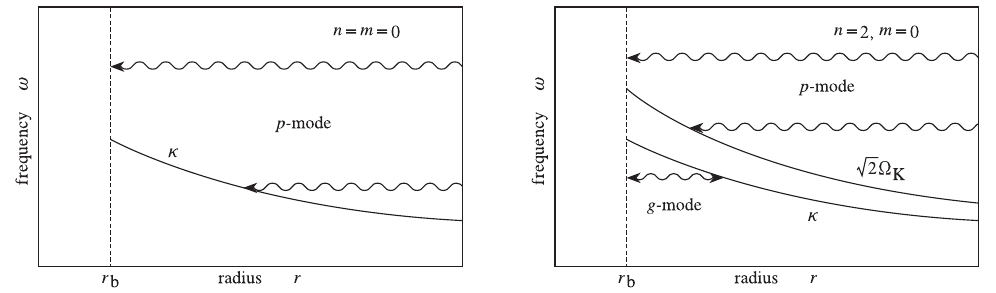
\includegraphics[scale=0.5]{waves.png}
\end{figure}



\subsection{Relativistic effects on the Dispersion Relation}

When general relativistic effects are taking into account 

\begin{equation}
\kappa^2 = \dfrac{GM}{r^3}\left( 1 + \dfrac{a}{\hat{r}^{3/2}}
\right)^{-2} \left(1 - \dfrac{6}{\hat{r}} + \dfrac{8a}{\hat{r}^{3/2}}
- \dfrac{3a^2}{\hat{r}^2}  \right)
\end{equation}

Where $a$ is a dimensionless parameter specifying the amount of
angular momentum of the central object if $a=0$ the object is rotating
and if $a=1$ the central object have the maximum rotation (the case of
extreme Kerr).

\begin{equation}
\hat{r} = \dfrac{r}{GM/c^2}
\end{equation}

\begin{equation}
\Omega_{}^2 = \Omega_{K}^2 \left(1 - \dfrac{4a}{\hat{r}^{3/2} +
\dfrac{3a^2}{\hat{r}^2}} \right)
\end{equation}

\begin{equation}
\Omega_K^2 = \dfrac{GM}{r^3} \left[ 1 + \dfrac{a}{(8
\hat{r}^3)^{1/2}}\right]^{-1}
\end{equation}

\begin{equation}
(\tilde{\omega}^2 + \kappa^2)(\tilde{\omega}^2 - n \Omega_{\bot}^2) =
\tilde{\omega}^2 c_s^2 k_{r}^2
\end{equation}

\begin{equation}
(\tilde{\omega}^2 - \kappa^2)(\tilde{\omega}^2 - n\Omega_{\bot}^2 ) =
\tilde{\omega}^2 c_s^2 k_r^2
\end{equation}

In Keplerian disks $\kappa \sim \Omega \sim \Omega_K$ and
$\Omega_{\bot}$ 

\begin{figure}
\centering
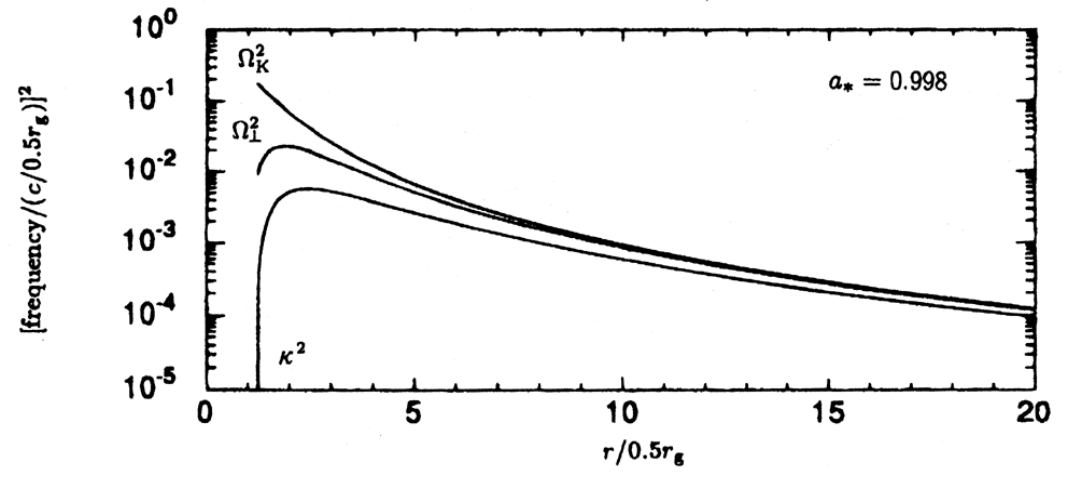
\includegraphics[scale=0.3]{relativsitc.png}
\end{figure}

\section{Low-Frequency Corrugation Waves:}

\begin{equation}
\omega \sim -\dfrac{1}{2} \Omega \dfrac{\Omega^2}{\Omega^2 -
\kappa^2} \dfrac{k_r^2 c_s^2 }{\Omega^2} + \dfrac{1}{2} \Omega
\dfrac{\Omega^2 - \Omega_{\bot}^2}{\Omega^2}
\end{equation}


\section{Trapped Oscillations in Relativistic Disks}

\subsection{Fundamental Mode}

For the fundamental mode $n=0$ the dispersion relation reduces to:

\begin{equation}
\omega^2 = \kappa^2 + c_s^2k_r^2
\end{equation}

This is the same dispersion relation for the non-relativistic
case but $\kappa$ is different see \verb+\ref{fig:X}+.
Because $k_r > 0$ the dispersion relation implies $\omega^2 >
\kappa^2$, The region in which this is satisfied is plotted in 
\verb+\ref{fig:X2}+. The propagation regions are three which
are explained as follows, In 1 the 


